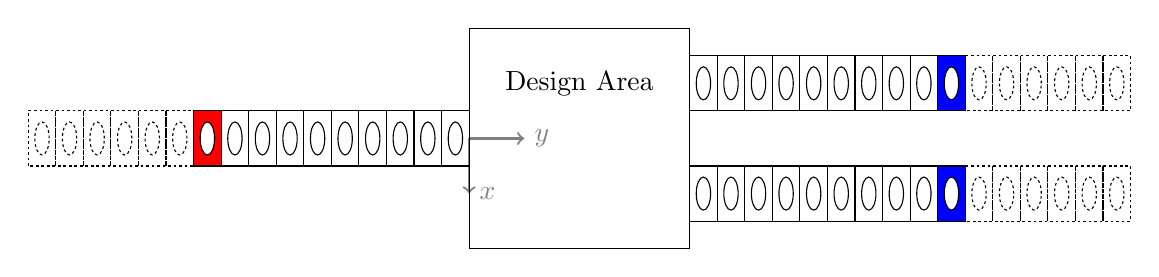
\begin{tikzpicture}[scale=0.7]
	\def \a{0.5}
	\def \w{1.0}
	\def \hx{0.13}
	\def \hy{0.3}
	\def \designx{4.0}
	\def \designy{4.0}
	\def \outputh{1.0}
	\def \nunitcells{16}
	\def \nnonpmls{10}

	% Coordinate system
	\draw[gray, thick, ->] (0,0) -- (0,-1) node [anchor=west] {$x$};
	\draw[gray, thick, ->] (0,0) -- (1,0) node [anchor=west] {$y$};

	% Input waveguide
	\begin{scope}[dash=on 1pt off 1pt phase 0pt]
		\foreach \ix [parse=true] in {-\nunitcells,...,-\nnonpmls-1} {
			\draw (\ix*\a, -0.5*\w) rectangle (\ix*\a + \a, 0.5*\w);
			\draw (\ix*\a + 0.5*\a, 0) circle [x radius=\hx, y radius=\hy];
		}
	\end{scope}
	\foreach \ix in {-\nnonpmls,...,-1} {
		\draw (\ix*\a, -0.5*\w) rectangle (\ix*\a + \a, 0.5*\w);
		\draw (\ix*\a + 0.5*\a, 0) circle [x radius=\hx, y radius=\hy];
	}
	\draw[fill=red] (-\nnonpmls*\a, -0.5*\w) rectangle (-\nnonpmls*\a+\a, 0.5*\w);
	%\node at (-\nnonpmls*\a + 0.5*\a, 0.5*\w) [anchor=south, red] {forward load};
	\draw[fill=white] (-\nnonpmls*\a + 0.5*\a, 0) circle [x radius=\hx, y radius=\hy];

	% Design area
	\draw (0, -\designx / 2) rectangle (\designy, \designx / 2);
	\node at (\designy / 2, 1) {Design Area};

	% Output waveguide
	\foreach \ix [parse=true] in {0, ..., \nnonpmls-1} {
		\draw (\designy + \ix*\a, \outputh - 0.5*\w) rectangle 
			  (\designy + \ix*\a + \a, \outputh + 0.5*\w);
		\draw (\designy + \ix*\a + 0.5*\a, \outputh)
			circle [x radius=\hx, y radius=\hy];

		\draw (\designy + \ix*\a, -\outputh - 0.5*\w) rectangle 
			  (\designy + \ix*\a + \a, -\outputh + 0.5*\w);
		\draw (\designy + \ix*\a + 0.5*\a, -\outputh)
			circle [x radius=\hx, y radius=\hy];
	}
	\begin{scope}[dash=on 1pt off 1pt phase 0pt]
		\foreach \ix [parse=true] in {\nnonpmls, ..., \nunitcells-1} {
			\draw (\designy + \ix*\a, \outputh - 0.5*\w) rectangle 
				  (\designy + \ix*\a + \a, \outputh + 0.5*\w);
			\draw (\designy + \ix*\a + 0.5*\a, \outputh)
				circle [x radius=\hx, y radius=\hy];

			\draw (\designy + \ix*\a, -\outputh - 0.5*\w) rectangle 
				  (\designy + \ix*\a + \a, -\outputh + 0.5*\w);
			\draw (\designy + \ix*\a + 0.5*\a, -\outputh)
				circle [x radius=\hx, y radius=\hy];
		}
	\end{scope}
	\draw[fill=blue] (\designy + \nnonpmls*\a - \a, \outputh-0.5*\w) rectangle
		(\designy + \nnonpmls*\a, \outputh + 0.5*\w);
	\draw[fill=white] (\designy + \nnonpmls*\a - 0.5*\a, \outputh) circle [x radius=\hx, y radius=\hy];
	\draw[fill=blue] (\designy + \nnonpmls*\a - \a, -\outputh-0.5*\w) rectangle
		(\designy + \nnonpmls*\a, -\outputh + 0.5*\w);
	\draw[fill=white] (\designy + \nnonpmls*\a - 0.5*\a, -\outputh) circle [x radius=\hx, y radius=\hy];


\end{tikzpicture}
